% Stellar Dominion: A Cathedral of Light on the Moon
% Design and Calculations Document
% Compile: pdflatex design-and-calculations.tex (run twice for references)

\documentclass[12pt,letterpaper]{article}

% ── Packages ──────────────────────────────────────────────────────────────────
\usepackage[margin=1.2in]{geometry}
\usepackage{amsmath,amssymb}
\usepackage{siunitx}
\usepackage{graphicx}
\usepackage{booktabs}
\usepackage{array}
\usepackage{hyperref}
\usepackage{xcolor}
\usepackage{listingsutf8}
\usepackage{fancyhdr}
\usepackage{titlesec}
\usepackage{microtype}
\usepackage{enumitem}
\usepackage{mdframed}
\usepackage{epigraph}
\usepackage[utf8]{inputenc}
\usepackage[T1]{fontenc}
\usepackage{concrete}   % Concrete Roman text (Zapf/Knuth Concrete Mathematics)
\usepackage{eulervm}    % Euler Virtual Math fonts

% ── Fix fancyhdr headheight ───────────────────────────────────────────────────
\setlength{\headheight}{14.5pt}

% ── Colors ────────────────────────────────────────────────────────────────────
\definecolor{emerald}{RGB}{0,160,100}
\definecolor{moonblue}{RGB}{20,40,80}
\definecolor{codebg}{RGB}{245,245,250}
\definecolor{codecomment}{RGB}{100,120,100}
\definecolor{codestring}{RGB}{160,40,40}
\definecolor{codekeyword}{RGB}{0,80,160}

% ── Hyperref setup ────────────────────────────────────────────────────────────
\hypersetup{
  colorlinks=true,
  linkcolor=moonblue,
  urlcolor=emerald,
  citecolor=moonblue,
  pdftitle={Stellar Dominion: A Cathedral of Light on the Moon},
  pdfauthor={Stellar Dominion Project},
}

% ── Section title formatting ──────────────────────────────────────────────────
\titleformat{\section}{\large\bfseries\color{moonblue}}{}{0em}{}[\color{emerald}\rule{\linewidth}{0.6pt}]
\titleformat{\subsection}{\normalsize\bfseries\color{moonblue}}{}{0em}{}

% ── Code listing style ─────────────────────────────────────────────────────────
\lstdefinestyle{python}{
  language=Python,
  backgroundcolor=\color{codebg},
  basicstyle=\footnotesize\ttfamily,
  commentstyle=\color{codecomment}\itshape,
  stringstyle=\color{codestring},
  keywordstyle=\color{codekeyword}\bfseries,
  numberstyle=\tiny\color{gray},
  numbers=left,
  stepnumber=5,
  numbersep=8pt,
  showstringspaces=false,
  breaklines=true,
  breakatwhitespace=true,
  frame=single,
  framerule=0.4pt,
  rulecolor=\color{emerald!50},
  captionpos=b,
  tabsize=4,
  keepspaces=true,
  columns=flexible,
  xleftmargin=14pt,
  extendedchars=true,
  literate=
    {✅}{{\checkmark}}1
    {—}{{---}}1
    {°}{{${}^\circ$}}1
    {×}{{$\times$}}1,
}

% ── Header / footer ───────────────────────────────────────────────────────────
\pagestyle{fancy}
\fancyhf{}
\fancyhead[L]{\small\color{moonblue}\textit{Stellar Dominion}}
\fancyhead[R]{\small\color{moonblue}\textit{Design \& Calculations}}
\fancyfoot[C]{\small\thepage}
\renewcommand{\headrulewidth}{0.3pt}

% ── Framed quote box ──────────────────────────────────────────────────────────
\newmdenv[
  topline=false, bottomline=false,
  rightline=false,
  linewidth=3pt,
  linecolor=emerald,
  backgroundcolor=emerald!5,
  innerleftmargin=12pt,
  innerrightmargin=12pt,
  innertopmargin=8pt,
  innerbottommargin=8pt,
  skipabove=12pt,
  skipbelow=12pt,
]{emeraldquote}

% ──────────────────────────────────────────────────────────────────────────────
\begin{document}

% ── Cover page (full-bleed visualization) ─────────────────────────────────────
\newgeometry{top=0pt,bottom=0pt,left=0pt,right=0pt}
\thispagestyle{empty}
\pagecolor{black}
\noindent\begin{minipage}[c][\paperheight][c]{\paperwidth}
  \centering
  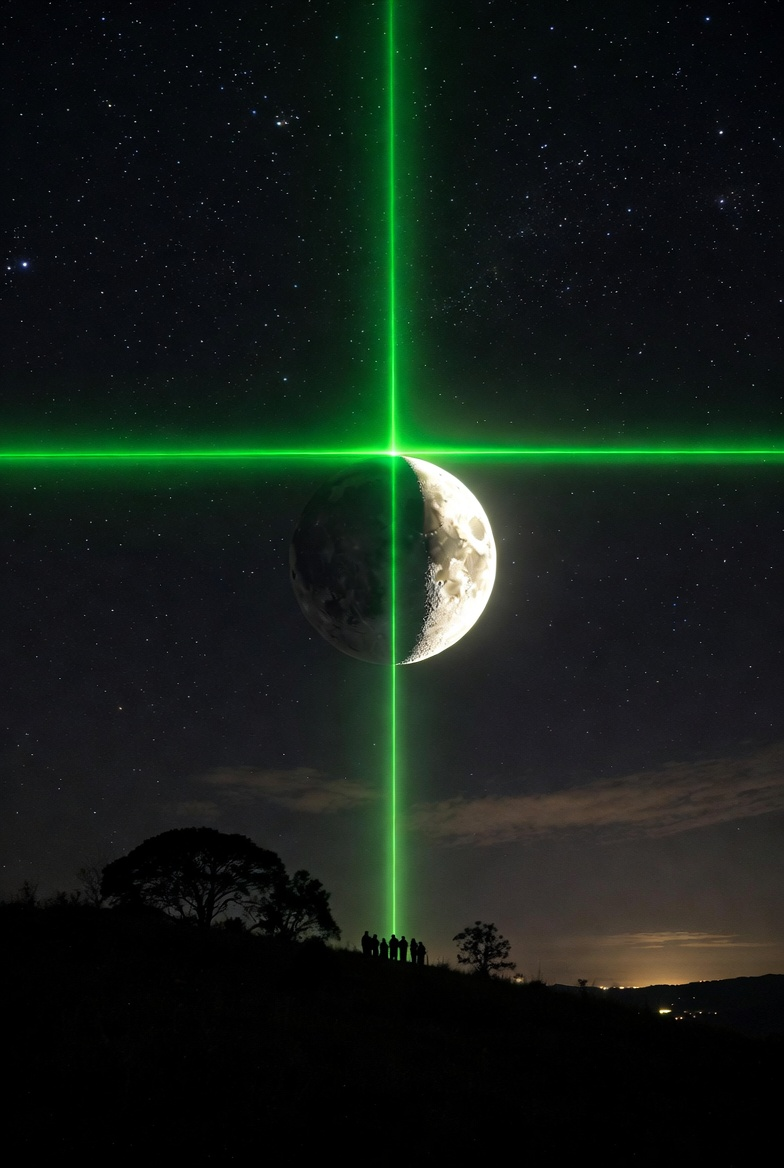
\includegraphics[width=\paperwidth,keepaspectratio=true]{images/lunar-cross-promo.jpeg}
\end{minipage}
\restoregeometry
\pagecolor{white}
\clearpage

% ── Title page ────────────────────────────────────────────────────────────────
\begin{titlepage}
  \centering
  \vspace*{2cm}
  {\color{moonblue}\rule{\linewidth}{1.5pt}}\\[0.4cm]
  {\Huge\bfseries\color{moonblue} Stellar Dominion}\\[0.3cm]
  {\large\color{emerald}\textit{A Cathedral of Light on the Moon}}\\[0.2cm]
  {\color{moonblue}\rule{\linewidth}{1.5pt}}\\[1.5cm]

  {\large\bfseries Projecting a Visible Emerald-Green Cross from the Moon's Northern Pole\\
  Visible Across the Entire Contiguous United States}\\[1.5cm]

  \begin{emeraldquote}
    \itshape For we are God's handiwork, created in Christ Jesus to do good works,
    which God prepared in advance for us to do.\\[0.3em]
    \normalfont\small\hfill---\,Ephesians 2:10 (NIV)
  \end{emeraldquote}

  \vfill

  {\small Design \& Calculations}\\[0.3cm]
  {\small Markus Fix}\\[0.3cm]
  {\small \today}
\end{titlepage}

% ── Abstract ──────────────────────────────────────────────────────────────────
\newpage
\begin{abstract}
\noindent
Stellar Dominion integrates a \SI{3}{\kilo\watt}--\SI{5}{\kilo\watt}
emerald-green fiber laser directly into a SpaceX Starship HLS that lands
permanently on the lunar north pole. The Starship becomes the operational base:
its \SI{50}{\meter} stainless steel hull provides structure, thermal mass, and
mounting area for SolAero IMM-\(\alpha\) solar panels. A deployable boom
extends the laser, telescope, and diffractive optical element from the top of
the vehicle, pointing horizontally toward Earth. The cross fires every Sunday
when the Moon is visible at night over the US, with aspirational first light on
Easter Sunday, April~1, 2027. Total system mass is \SI{1.4}{\tonne}---a 39\%
reduction over a standalone pallet design. Core project cost is
\$42--114 million (projector, energy system, Starship modifications, and
ground systems), with a Starship lunar cargo flight adding \$20--50 million
if purchased separately. Total lifecycle cost including launch and ten years
of operations is \$72--192 million.
\end{abstract}

\tableofcontents
\newpage

% ─────────────────────────────────────────────────────────────────────────────
\section{A Cathedral on the Moon}
% ─────────────────────────────────────────────────────────────────────────────

For as long as we have existed, humanity has looked up at the Moon and dreamed.
Every civilization, every culture, every solitary soul on a dark night has felt
the pull of that pale light. Now imagine changing what they see.

Standing anywhere in the continental United States on a clear night, you look
up at the full Moon. And there---unmistakable, luminous, impossible to
ignore---a brilliant \textbf{\color{emerald}emerald-green cross} burns above
the lunar disk. Not a projection on a building. Not a screen. A real structure,
\SI{384400}{\kilo\meter} away, painting the sky with coherent light.

\textbf{Stellar Dominion} proposes building a cathedral on the Moon's northern
pole---not a cathedral of worship, but of engineering. Inside it: a
kilowatt-class laser and diffractive optics that project a cross-shaped beam
across the Earth--Moon divide, blanketing all 48 contiguous states in a single,
shared, naked-eye spectacle.

\begin{emeraldquote}
  \textbf{One beam. One Moon. 330 million people looking up at the same light.}
\end{emeraldquote}

This is not science fiction. Every component---the laser, the optics, the power
system, the launch vehicle---exists today or is in active commercial
development. What is missing is the will to build something this audacious.

\subsection{Mission Parameters at a Glance}

\begin{center}
\begin{tabular}{ll}
\toprule
\textbf{Parameter} & \textbf{Value} \\
\midrule
Platform & SpaceX Starship HLS (permanent installation) \\
Location & Lunar north pole (peak of eternal light) \\
Target coverage & Contiguous United States (lower 48 states) \\
Cross pattern & \ang{0.7} total angular span, \SI{532}{\nano\meter} green \\
Optical power & \SI{3}{\kilo\watt}--\SI{5}{\kilo\watt} \\
Power source & SolAero IMM-\(\alpha\), \SI{50}{\meter\squared}, \SI{21.8}{\kilo\watt} peak \\
System mass & \SI{1.4}{\tonne} \\
Operation & Sundays only; first light Easter 2027 \\
Design life & 10 years \\
Core project cost (excl.\ launch) & \$42--114 million \\
Total lifecycle cost (incl.\ launch + ops) & \$72--192 million \\
\bottomrule
\end{tabular}
\end{center}

% ─────────────────────────────────────────────────────────────────────────────
\section{System Architecture}
% ─────────────────────────────────────────────────────────────────────────────

The Stellar Dominion hardware integrates directly into a SpaceX Starship HLS
that lands permanently on the lunar north pole. The Starship is not merely the
delivery vehicle---it \emph{is} the operational platform. No separate structure
is required. All subsystems are either passive or software-controlled; no
human presence is needed after commissioning.

\subsection{What Starship Provides for Free}

\begin{center}
\begin{tabular}{ll}
\toprule
\textbf{Resource} & \textbf{Benefit} \\
\midrule
50\,m stainless steel hull & Structure, rigidity, mounting surface \\
Height & 13\,km horizon line-of-sight; clears local terrain \\
Thermal mass ($>$200 t steel) & Stabilises laser operating temperature \\
Power bus & Shared Starship HLS infrastructure \\
Comms & S-band/Ku-band supplemented by minimal custom avionics \\
Structural durability & Stainless steel in vacuum; effectively indefinite life \\
\bottomrule
\end{tabular}
\end{center}

\subsection{Stellar Dominion Subsystems}

\begin{center}
\begin{tabular}{lll}
\toprule
\textbf{Subsystem} & \textbf{Function} & \textbf{Key spec} \\
\midrule
Fiber laser & Generate green light & \SI{5}{\kilo\watt} optical, \SI{532}{\nano\meter} \\
Beam expander & Collimate to \SI{\sim 0.5}{\meter} aperture & M$^2 < 1.2$ \\
DOE & Shape beam into cross pattern & \ang{0.7} span, 80\% efficiency \\
Deployable boom & Position optics above hull & 3--5\,m carbon composite + gimbal \\
Solar array & Primary power & \SI{50}{\meter\squared} SolAero IMM-$\alpha$, \SI{20}{\kilo\watt} \\
Battery bank & Eclipse bridging & \SI{325}{\kilo\gram} Amprius Si-anode \\
Radiator panels & Reject laser waste heat & \SI{20}{\meter\squared}, hull-mounted \\
Pointing assembly & Track Earth as Moon orbits & $< \ang{0.1}$ accuracy \\
Avionics + comms & Housekeeping, telemetry & Minimal custom; shares Starship \\
\bottomrule
\end{tabular}
\end{center}

% ─────────────────────────────────────────────────────────────────────────────
\section{Optical Design}
% ─────────────────────────────────────────────────────────────────────────────

\subsection{Laser}

Green light at \SI{532}{\nano\meter} sits at the peak of the human photopic
response curve, maximizing perceived brightness per watt delivered.
\textbf{Important clarification:} high-power fiber lasers such as the IPG YLS
series operate at \SI{1070}{\nano\meter} infrared. Reaching \SI{532}{\nano\meter}
requires a \textbf{second-harmonic generation (SHG)} crystal stage---a well-established
nonlinear optical process, but one that requires custom engineering at the 5\,kW CW level.
CW SHG conversion efficiency is typically 60--80\%, yielding a combined wall-plug efficiency
of $\approx$25--35\% (baseline: 30\%). This is an engineering development task, not a COTS
solution.

\begin{center}
\begin{tabular}{ll}
\toprule
\textbf{Parameter} & \textbf{Value} \\
\midrule
Wavelength & \SI{532}{\nano\meter} (SHG from \SI{1064}{\nano\meter} IR fiber laser) \\
Optical output & \SI{3}{\kilo\watt}--\SI{5}{\kilo\watt} CW \\
Wall-plug efficiency & 25--35\% (baseline: 30\%, including SHG stage) \\
Electrical power & \SI{12}{\kilo\watt}--\SI{20}{\kilo\watt} \\
Beam quality & $M^2 < 1.2$ \\
Rated lifetime & $> \num{100000}$ hours ($\approx$ 11 years) \\
Mass (including SHG) & \SI{200}{\kilo\gram}--\SI{300}{\kilo\gram} \\
\bottomrule
\end{tabular}
\end{center}

\subsection{Radiometric Power Requirement}

The cross must be bright enough to see with the naked eye against the night sky.
We target an irradiance at Earth equivalent to a naked-eye magnitude $\approx 0$
green source:

\[
  E_{\min} \approx \SI{1e-9}{\watt\per\meter\squared}
\]

The cross consists of two arms, each \ang{0.7} long and \ang{0.05} thick. The
solid angle of each arm is:

\[
  \Omega_{\text{arm}} = \left(\ang{0.7} \times \frac{\pi}{\ang{180}}\right)
                       \times \left(\ang{0.05} \times \frac{\pi}{\ang{180}}\right)
                      = 1.06 \times 10^{-5}\ \si{\steradian}
\]

Total solid angle of the cross (two arms, minus small central overlap):

\[
  \Omega_{\text{cross}} = 2 \times 1.06 \times 10^{-5}
                        \approx \mathbf{2.05 \times 10^{-5}\ \si{\steradian}}
\]

Required optical power, using the inverse-square radiometric relation:

\[
  \boxed{P_{\text{opt}} = E \cdot \Omega \cdot d^2}
\]

\[
  d^2 = \left(3.844 \times 10^8\ \si{\meter}\right)^2
       = 1.477 \times 10^{17}\ \si{\meter\squared}
\]

\[
  P_{\text{opt}} = (10^{-9})\cdot(2.05 \times 10^{-5})\cdot(1.477 \times 10^{17})
                \approx \SI{3.0}{\kilo\watt}
\]

With \SI{5}{\kilo\watt} deployed we operate with a comfortable 4.5\,dB margin
above threshold---allowing for optical losses, DOE efficiency, and atmospheric
absorption.

\subsection{Diffractive Optical Element}

A diffractive optical element (DOE) is a thin phase-modulating optic that
reshapes the incident Gaussian laser beam into an arbitrary far-field intensity
pattern---in our case, a cross. The phase mask is computed using the
\textbf{Gerchberg--Saxton} iterative Fourier algorithm~\cite{GS1972}, which
alternately applies the target amplitude constraint in the far field and the
physical constraint (unit amplitude) in the near field until convergence.

The DOE is a passive optical component: once manufactured, it requires no
power, has no moving parts, and suffers no degradation in vacuum. A
surface-relief fused-silica DOE achieves 80--95\% diffraction efficiency.

The algorithm is already prototyped in this project. The DOE pattern generator
is listed in Section~\ref{sec:code-doe}.

\subsection{Angular Geometry}

\begin{center}
\begin{tabular}{ll}
\toprule
\textbf{Quantity} & \textbf{Value} \\
\midrule
Earth--Moon distance $d$ & \SI{384400}{\kilo\meter} \\
Continental US east--west span & \SI{4500}{\kilo\meter} \\
US angular width $\theta_{\text{US}}$ & $\arctan\!\left(\frac{4500}{384400}\right) \approx \ang{0.67}$ \\
Cross total span & \ang{0.7} (covers US with margin) \\
Cross arm thickness & \ang{0.05} \\
Moon apparent diameter & \ang{0.5} \\
\bottomrule
\end{tabular}
\end{center}

% ─────────────────────────────────────────────────────────────────────────────
\section{Power System}
% ─────────────────────────────────────────────────────────────────────────────

\subsection{Landing Site: Peaks of Eternal Light}

The lunar north pole hosts several elevated ridges and crater rims that receive
near-continuous sunlight throughout the lunar year---nicknamed ``peaks of
eternal light.'' The rim of Peary crater ($88.6\,^\circ$N) and adjacent
ridgelines identified by NASA's Lunar Reconnaissance Orbiter (LRO) illumination
maps receive sunlight $70$--$95\%$ of the time, with eclipse periods of hours
at most during lunar winter.

The solar constant at the Moon equals that at Earth (no atmosphere to
attenuate): $G_{\odot} = \SI{1361}{\watt\per\meter\squared}$.

\subsection{Solar Array: Rocket Lab (SolAero) IMM-\texorpdfstring{$\alpha$}{alpha}}

Operating in vacuum with no weather or oxidation, we use \textbf{bare}
IMM-$\alpha$ (inverted metamorphic multi-junction) cells on lightweight Kapton
substrate---no cover glass required~\cite{SolAero}. These cells are
manufactured by Rocket Lab Space Systems, which acquired SolAero Technologies
in 2022, and are commercially available through an established procurement
path. This eliminates the largest single mass item in traditional space solar
arrays.

\begin{center}
\begin{tabular}{ll}
\toprule
\textbf{Parameter} & \textbf{Value} \\
\midrule
Technology & SolAero IMM-$\alpha$, bare cells on Kapton \\
Cell efficiency & 32\% (AM0, beginning of life) \\
Areal density & \SI{2}{\kilo\gram\per\meter\squared} deployed \\
Deployment & Rollout panels unfurling from Starship hull \\
\bottomrule
\end{tabular}
\end{center}

\begin{align}
  P_{\text{required}} &\approx \SI{20}{\kilo\watt} \quad \text{(see power budget)} \\
  \eta_{\text{cell}}  &= 0.32 \quad \text{(SolAero IMM-$\alpha$, BOL)} \\
  P_{\text{array}}    &= G_{\odot} \cdot \eta \cdot A
    = 1361 \times 0.32 \times A = 435\, A\ \si{\watt\per\meter\squared}
\end{align}

Setting $P_{\text{array}} \geq \SI{20}{\kilo\watt}$ (with degradation margin):

\[
  A = \frac{20\,000}{435} \approx \SI{46.0}{\meter\squared}
    \quad \rightarrow \quad \textbf{baseline: \SI{50}{\meter\squared},\ \SI{100}{\kilo\gram}}
\]

\noindent This compares to \SI{500}{\kilo\gram} for traditional rigid panels
at \SI{10}{\kilo\gram\per\meter\squared}---a \textbf{5$\times$ mass
reduction}.

\medskip
\noindent \textbf{Upgrade path.} Rocket Lab's next-generation
\textbf{IMM-$\boldsymbol\beta$} cell achieves 33.3\% efficiency with improved
specific power (W/kg). It is a drop-in replacement for IMM-$\alpha$ requiring
no redesign of the array structure or power system. If available at mission
procurement time, IMM-$\beta$ would provide additional degradation margin at no
mass penalty.

\subsection{Battery Technology: Amprius Silicon-Anode}

We baseline \textbf{Amprius SiCore} silicon-anode lithium-ion cells---the
highest energy-density Li-ion cells commercially available. Amprius already
ships to aerospace and defense customers~\cite{Amprius}.

\begin{center}
\begin{tabular}{llp{5cm}}
\toprule
\textbf{Level} & \textbf{Energy density} & \textbf{Notes} \\
\midrule
Cell & \SI{400}{\watt\hour\per\kilo\gram} & Amprius SiCore, shipping \\
Pack (custom vacuum-rated) & $\sim$\SI{280}{\watt\hour\per\kilo\gram} & 70\% cell-to-pack; radiative cooling, composite enclosure, BMS \\
\bottomrule
\end{tabular}
\end{center}

\subsection{Battery Sizing (Eclipse Bridging)}

LRO illumination models for Peary crater rim show worst-case darkness periods of
\textbf{up to 120--124 hours} ($\approx$5 Earth days) during some lunar winters.
The laser shuts down during eclipses (no observer sees an eclipsed Moon). Battery
sustains avionics and thermal survival only, in two modes:

\begin{center}
\begin{tabular}{lll}
\toprule
\textbf{Mode} & \textbf{Load} & \textbf{Conditions} \\
\midrule
Full survival & $\sim$\SI{1}{\kilo\watt} & Short eclipses ($\leq$72\,hr): full avionics + heaters \\
Hibernation & $\sim$\SI{500}{\watt} & Extended eclipses ($>$72\,hr): battery heat + avionics keep-alive \\
\bottomrule
\end{tabular}
\end{center}

The system uses ephemeris to predict eclipse duration before entry and selects the
appropriate mode. Battery capacity (unchanged):

\[
  E_{\text{capacity}} = \SI{90}{\kilo\watt\hour}
  \quad \rightarrow \quad E_{\text{usable}} = 90 \times 0.80 = \SI{72}{\kilo\watt\hour}
\]

\[
  \text{At \SI{500}{\watt} (hibernation):}\quad
  \frac{72\,000}{500} = \SI{144}{\hour} > \SI{124}{\hour}\ \checkmark
\]

At \SI{280}{\watt\hour\per\kilo\gram} pack-level (Amprius):

\[
  m_{\text{battery}} = \frac{90\,000}{280} = \SI{321}{\kilo\gram}
    \quad \rightarrow \quad \textbf{baseline: \SI{325}{\kilo\gram}}
\]

\subsection{Power Budget}

\begin{center}
\begin{tabular}{lrr}
\toprule
\textbf{Subsystem} & \textbf{Power (W)} & \textbf{Notes} \\
\midrule
Fiber laser @ 30\% efficiency (incl.\ SHG) & 17\,000 & Dominant load \\
Pointing assembly & 200 & Low-power servo drives \\
Avionics + communications & 300 & Housekeeping, telemetry \\
Thermal heaters & 500 & Laser pre-heating during cold periods \\
10\% margin & 1\,800 & \\
\midrule
\textbf{Total} & \textbf{19\,800} & $\approx$\,\SI{20}{\kilo\watt} \\
\bottomrule
\end{tabular}
\end{center}

% ─────────────────────────────────────────────────────────────────────────────
\section{Thermal Management}
% ─────────────────────────────────────────────────────────────────────────────

\subsection{Waste Heat}

The laser subsystem (IR source + SHG stage) produces 12\,kW of waste heat
(electrical input minus optical output). Combined with avionics, total heat
rejection is:

\[
  Q_{\text{total}} = P_{\text{elec}} - P_{\text{opt}} + P_{\text{avionics}}
                   \approx 17\,000 - 5\,000 + 500 = \SI{12.5}{\kilo\watt}
\]

\subsection{Radiator Sizing}

In lunar vacuum, heat can only be rejected by radiation. From the
Stefan--Boltzmann law:

\[
  Q = \varepsilon \cdot \sigma \cdot A \cdot \left(T_{\text{rad}}^4
    - T_{\text{env}}^4\right)
\]

where $\varepsilon = 0.85$ (black anodized aluminum), $\sigma =
\SI{5.67e-8}{\watt\per\meter\squared\per\kelvin\tothe{4}}$, $T_{\text{rad}} =
\SI{340}{\kelvin}$ (laser operating temp), and $T_{\text{env}} =
\SI{100}{\kelvin}$ (polar sky background, conservative):

\[
  \frac{Q}{A} = 0.85 \times 5.67 \times 10^{-8}
                \times \left(340^4 - 100^4\right)
              \approx \SI{640}{\watt\per\meter\squared}
\]

\[
  A_{\text{radiator}} = \frac{12\,500}{640} \approx \SI{19.5}{\meter\squared}
    \quad \rightarrow \quad \textbf{baseline: \SI{20}{\meter\squared}}
\]

% ─────────────────────────────────────────────────────────────────────────────
\section{Mass Budget}
% ─────────────────────────────────────────────────────────────────────────────

\begin{center}
\begin{tabular}{lrp{5.5cm}}
\toprule
\textbf{Subsystem} & \textbf{Mass (kg)} & \textbf{Basis} \\
\midrule
Fiber laser assembly (incl.\ SHG) & 280 & IPG YLS class + SHG crystal assembly, space-qualified \\
DOE + beam optics & 200 & 0.5\,m aperture, lightweight mirror \\
Solar array (50\,m$^2$, SolAero IMM-$\alpha$) & 100 & 2\,kg/m$^2$, bare cells on Kapton \\
Battery bank (Amprius Si-anode) & 325 & 90\,kWh @ 280\,Wh/kg pack \\
Radiator panels (20\,m$^2$, hull-mounted) & 100 & Flush on Starship hull \\
Pointing assembly & 100 & Star tracker + 2-axis gimbal \\
Avionics + communications & 40 & Minimal custom; shares Starship comms \\
Deployable boom (3--5\,m) & 75 & Carbon composite + gimbal interface \\
\textit{Structure/pallet} & \textit{0} & \textit{Eliminated --- Starship IS the structure} \\
15\% integration margin & 183 & \\
\midrule
\textbf{Total} & \textbf{1\,403} & \textbf{$\approx$\,1.4 tonnes} \\
\bottomrule
\end{tabular}
\end{center}

\noindent At \SI{1.4}{\tonne}---a 39\% reduction over the standalone pallet
architecture---the Stellar Dominion hardware is a small fraction of Starship
HLS delivery capacity. The mass savings stem from eliminating the pallet
structure entirely (\SI{400}{\kilo\gram}) and from SolAero's 5$\times$
lighter solar panels (\SI{100}{\kilo\gram} vs.\ \SI{500}{\kilo\gram}).

% ─────────────────────────────────────────────────────────────────────────────
\section{Landing, Deployment, and Pointing}
% ─────────────────────────────────────────────────────────────────────────────

\subsection{Landing Site}

Target: rim of Peary crater ($88.6\,^\circ$N) or an adjacent ridgeline with
confirmed $>70\%$ solar illumination per LRO illumination maps. Starship HLS
employs terrain-relative navigation (TRN) for metre-scale landing accuracy.

\textbf{Starship stays permanently.} After touchdown, the engines shut down
and the vehicle becomes the operational platform. There is no departure.

\textbf{Height advantage.} With the laser system at $\sim$\SI{50}{\meter}
(near the top of Starship), the geometric line-of-sight to the horizon is:

\[
  d_{\text{horizon}} = \sqrt{2 R_{\text{Moon}} h}
    = \sqrt{2 \times 1\,737\,400 \times 50}
    \approx \SI{13.2}{\kilo\meter}
\]

This comfortably clears local terrain, reducing sensitivity to the exact
landing position within the polar region.

\subsection{Deployment Sequence}

\begin{enumerate}[leftmargin=1.5em]
  \item Starship lands at polar peak (pre-surveyed via LRO); engines shut down permanently
  \item SolAero panels unfurl from hull exterior; battery begins charging
  \item System boots from Starship power bus; self-check; Earth comm link established
  \item Star tracker acquires attitude; JPL ephemeris loaded via uplink
  \item Deployable boom extends from nosecone area; laser/optics at operational position
  \item Laser fires at 10\% power; Earth ground station confirms pointing
  \item Full-power commissioning; cross pattern confirmed
  \item \textbf{First Light} --- system enters autonomous Sunday operation schedule
\end{enumerate}

Estimated commissioning time: 2--4 weeks post-landing.

\subsection{Long-Term Structural Durability}

Starship's 304L stainless steel hull is well-suited to permanent lunar
deployment: no corrosion (no oxygen or moisture), mild polar thermal cycling
($\sim$\SI{50}{\kelvin} vs.\ \SI{300}{\kelvin} at equatorial sites), and no
wind, seismic, or weather loading. Structural design life exceeds the
10-year mission life by a large margin.

\subsection{Lunar Surface Environment}

\subsubsection*{Landing Plume and Dust}

Starship's descent engines displace loose regolith during landing. In
vacuum, displaced particles follow \textbf{ballistic trajectories}---there is
no lingering cloud (no atmosphere to suspend particles), and ejecta settles
within seconds of engine shutdown. All sensitive surfaces (solar panels,
optics, DOE) are stowed in protective enclosures during landing and deployed
only after the plume has fully dispersed.

Once deployed, there is \textbf{no ongoing aeolian transport}---without an
atmosphere, surface material cannot be re-mobilized by wind. Electrostatic
dust levitation exists near the terminator but produces negligible mass flux
at \SI{50}{\meter} elevation. Anti-static surface coatings on optical
elements are a prudent precaution. Micrometeorite-driven regolith gardening
produces a very low secondary ejecta flux over 10 years---relevant for
surface abrasion studies but not a mission-level concern for fused-silica
optics.

\subsubsection*{Radiation Environment}

The Moon has no magnetosphere. The system is continuously exposed to galactic
cosmic rays (GCR) and sporadic solar particle events (SPE). Mitigations:

\begin{itemize}[leftmargin=1.5em]
  \item Starship's $\sim$4\,mm stainless steel hull provides $\approx$5--10\,g/cm$^2$
        of areal shielding for internally mounted electronics, attenuating
        the lower-energy SPE proton spectrum.
  \item Laser diodes and SHG crystal are inside the boom enclosure with
        additional local shielding.
  \item Sunday-only operation limits cumulative dose to active electronics
        ($\approx$416 operating hours/year vs.\ 8\,760 for continuous
        operation).
  \item Avionics baseline: radiation-hardened design (latch-up tolerant,
        EDAC on memory)---standard for lunar surface missions.
\end{itemize}

\noindent \textbf{Open item:} A dedicated radiation transport analysis
(SHIELDOSE or equivalent) is needed to quantify worst-case SPE fluence
and size any additional local shielding for the avionics enclosure.

\subsection{Pointing and Tracking}

The laser must track the continental United States
($38\,^\circ$N,\;$97\,^\circ$W) as the Moon orbits Earth and Earth rotates.

\textbf{Earth is always near the horizon.} From the lunar north pole, Earth sits
at $0\,^\circ$ elevation ($\pm\ang{6.7}$ with libration in latitude). The
boom-mounted gimbal therefore points roughly horizontally---a geometrically
simple configuration that clears the vehicle body without requiring an overhead
slew. As Earth drifts slowly across the horizon driven by libration, the gimbal
compensates with a gentle elevation adjustment well within its travel range.

\begin{center}
\begin{tabular}{lll}
\toprule
\textbf{Component} & \textbf{Spec} & \textbf{Heritage} \\
\midrule
Star tracker & $< \ang{;;5}$ accuracy & Jena-Optronik Astro APS class \\
2-axis gimbal & $\ang{0.004}$/s max slew rate needed & Commercial industrial \\
Ephemeris & JPL DE430 & Pre-loaded + uplink corrections \\
Update rate & \SI{1}{\hertz} & Earth moves $\ang{0.004}$/s in lunar sky \\
Required accuracy & $< \ang{0.1}$ & Cross arm is \ang{0.7} wide \\
\bottomrule
\end{tabular}
\end{center}

% ─────────────────────────────────────────────────────────────────────────────
\section{Visibility Analysis}
% ─────────────────────────────────────────────────────────────────────────────

\subsection{Conditions for Visibility}

Three conditions must be simultaneously satisfied for a US observer to see the
cross:
\begin{enumerate}
  \item The Moon is \textbf{above the horizon} at the observer's location
  \item It is \textbf{night} (astronomical twilight or darker)
  \item The Moon is in a \textbf{gibbous or full phase}---sufficient illumination
        for the Moon to be a landmark, and sky dark enough for the cross to pop
\end{enumerate}

\subsection{Lunar Libration and North Pole Visibility}

The laser sits at the Moon's north pole. From Earth, the north pole is visible
at an angle that varies with \emph{libration in latitude}: the Moon nods
$\pm\ang{6.7}$ over its $\approx 27$-day orbit. When libration tilts the pole
toward Earth, the cross projector has maximum line-of-sight exposure. Even when
tilted away, the beam geometry is unchanged---the cross still covers the US.

\subsection{Monthly Visible Hours (Mid-Latitude US Observer)}

\begin{center}
\begin{tabular}{llrr}
\toprule
\textbf{Phase} & \textbf{Sky condition} & \textbf{Hours/night} & \textbf{Nights/month} \\
\midrule
Full Moon & Best; brilliant cross on dark sky & $\sim$6 & $\sim$3 \\
Waxing/waning gibbous & Good & 4--8 & $\sim$8 \\
Quarter & Marginal (competing twilight glow) & $\sim$4 & $\sim$4 \\
Crescent & Poor & $<$2 & few \\
\midrule
\multicolumn{2}{l}{\textbf{Useful viewing hours per month}} & \multicolumn{2}{r}{\textbf{$\approx$\,30--50 hours}} \\
\bottomrule
\end{tabular}
\end{center}

The cross is most spectacular at full Moon---when all 330 million Americans can
look up simultaneously and see the same light.

% ─────────────────────────────────────────────────────────────────────────────
\section{Sunday Operation Mode}
% ─────────────────────────────────────────────────────────────────────────────

The baseline design supports continuous autonomous operation, but the cross
fires \textbf{only on Sundays}---when the Moon is visible at night over the
United States. This is a scheduling decision, not a hardware redesign: the
same \SI{50}{\meter\squared} SolAero array and \SI{325}{\kilo\gram} Amprius
battery are retained.

\subsection{Why Not Shrink the Hardware?}

One might propose a smaller solar array ($\sim$\SI{7}{\meter\squared}) that
charges a larger battery all week, discharging on Sunday. With SolAero panels
at \SI{2}{\kilo\gram\per\meter\squared}, the baseline wins decisively:

\begin{center}
\begin{tabular}{lrrr}
\toprule
\textbf{Architecture} & \textbf{Solar (kg)} & \textbf{Battery (kg)} & \textbf{Total (kg)} \\
\midrule
Baseline (50\,m$^2$ SolAero + survival battery) & 100 & 325 & 425 \\
Small solar + burst battery (7\,m$^2$ SolAero) & 14 & 675 & 689 \\
\bottomrule
\end{tabular}
\end{center}

\noindent The baseline is \textbf{264\,kg lighter}---the opposite of a wash.
SolAero's low areal density makes large arrays cheap on mass, so the
week-long charging strategy loses its mass incentive entirely. It also adds
single-point failure risk and deep cycling stress. The baseline hardware is
kept as-is.

\subsection{Benefits of Sunday-Only Operation}

\begin{center}
\begin{tabular}{lp{8cm}}
\toprule
\textbf{Benefit} & \textbf{Impact} \\
\midrule
Laser lifetime & $\sim$416 hrs/year vs.\ 8{,}760 $\to$ effectively indefinite ($>$240 years at rated 100{,}000 hrs) \\
Thermal cycling & Reduced stress on optics and laser diodes \\
Ground operations & Sunday-only monitoring saves \$5--10M over 10 years \\
Narrative resonance & The cross appears on the Sabbath; Easter Sunday is the natural inaugural event \\
\bottomrule
\end{tabular}
\end{center}

% ─────────────────────────────────────────────────────────────────────────────
\section{Cost Estimates}
% ─────────────────────────────────────────────────────────────────────────────

All figures in 2025 USD. Ranges reflect uncertainty between COTS and
space-qualified component pricing (typically $5\times$--$20\times$ premium for
space qualification).

\begin{center}
\begin{tabular}{lrrl}
\toprule
\textbf{Item} & \textbf{Low (\$M)} & \textbf{High (\$M)} & \textbf{Basis} \\
\midrule
\multicolumn{4}{l}{\textit{Core Project --- projector, energy system, Starship modifications}} \\
\midrule
Laser system (5\,kW, space-qual) & 5 & 15 & \$200--500/W; 5--20$\times$ space premium \\
DOE + beam optics & 2 & 5 & Custom fused-silica DOE + telescope \\
Solar array (50\,m$^2$, SolAero IMM-$\alpha$) & 5 & 12 & Premium cells; less area than traditional \\
Battery bank (Amprius Si-anode) & 3 & 8 & 325\,kg; COTS cells + custom space pack \\
Radiators + thermal hardware & 1 & 2 & Hull-mounted; standard spacecraft thermal \\
Pointing assembly + boom & 3 & 8 & Star tracker, 2-axis gimbal, carbon boom \\
Avionics + communications & 1 & 3 & Minimal custom; shares Starship S-band \\
Starship modifications + integration & 3 & 8 & Hull/power/comms interfaces with SpaceX \\
System integration \& test & 8 & 20 & Thermal-vac, vibration, EMI \\
Ground station setup & 3 & 8 & Antenna, control software \\
Project management + contingency & 8 & 25 & 15--20\% of hardware cost \\
\midrule
\textit{Core project subtotal} & \textit{42} & \textit{114} & \textit{without launch} \\
\midrule
\multicolumn{4}{l}{\textit{Launch \& Delivery}} \\
\midrule
Starship lunar cargo flight & 20 & 50 & SpaceX projected lunar cargo pricing \\
\midrule
\textbf{Grand total} & \textbf{62} & \textbf{164} & \textbf{$\approx$\,\$60--165M} \\
\bottomrule
\end{tabular}
\end{center}

\noindent The core project---the projector, energy system, and Starship
modifications---costs \textbf{\$42--114M}. Launch is a separable line item:
if the hardware rides to the Moon as manifested cargo on a Starship flight
that is flying anyway, the incremental launch cost is zero. Even paying the
full dedicated flight, the complete mission fits within the budget of a
medium-class space mission.

\medskip
\noindent For perspective: the Hubble Space Telescope cost approximately
\$1.5\,billion in 1990 dollars. A single NASA CLPS lunar lander contract
costs \$100--400\,M. Stellar Dominion is achievable for the cost of one CLPS
contract---and would be seen by orders of magnitude more people.

% ─────────────────────────────────────────────────────────────────────────────
\section{Operational Lifetime and Costs}
% ─────────────────────────────────────────────────────────────────────────────

\subsection{Component Lifetimes}

\begin{center}
\begin{tabular}{llp{5.5cm}}
\toprule
\textbf{Component} & \textbf{Rated Life} & \textbf{Notes} \\
\midrule
Fiber laser & $>$100\,000 hours ($\approx$11 years) & Sunday-only: $\sim$416 hrs/yr $\to$ indefinite \\
Solar array & 15--20 years & 1--3\%/year radiation degradation \\
Amprius Si-anode battery & 1\,000--2\,000 cycles & Sunday-only cycling extends life well beyond 10 years \\
Avionics & 10--15 years & Radiation-hardened design \\
DOE (passive optic) & Indefinite & No moving parts; vacuum-stable \\
Pointing gimbal & 7--10 years & Wear item; oversize for life margin \\
\bottomrule
\end{tabular}
\end{center}

\textbf{Mission design life: 10 years.}

\subsection{Annual Operating Costs (Sunday Operation Mode)}

\begin{center}
\begin{tabular}{lrr}
\toprule
\textbf{Item} & \textbf{Low (\$/yr)} & \textbf{High (\$/yr)} \\
\midrule
Ground station ops (Sunday + weekly health) & 500\,000 & 1\,500\,000 \\
Mission operations team (1--3 FTE) & 300\,000 & 800\,000 \\
Ephemeris updates + uplink & 50\,000 & 200\,000 \\
Contingency & 150\,000 & 300\,000 \\
\midrule
\textbf{Annual total} & \textbf{1\,000\,000} & \textbf{2\,800\,000} \\
\bottomrule
\end{tabular}
\end{center}

\noindent Ten-year operating cost: approximately \$10--28\,M.

\medskip
\noindent \textbf{Core project + 10 years ops (no launch): \$52--142 million.}

\noindent \textbf{Full lifecycle (core + Starship flight + 10 years ops):
\$72--192 million.}

% ─────────────────────────────────────────────────────────────────────────────
\section{Project Timeline}
% ─────────────────────────────────────────────────────────────────────────────

\textbf{Aspirational first light: Easter Sunday, April 1, 2027.}

\medskip
\noindent Working backward: first light on Easter requires launch by early March
2027, payload integration by mid-February, and a 10-month compressed build
starting April 2026. Compression is achieved by ordering the laser at kickoff,
overlapping integration with late hardware deliveries, and running
thermal-vacuum and vibration tests in parallel.

\begin{center}
\begin{tabular}{clp{7cm}}
\toprule
\textbf{Month} & \textbf{Milestone} & \textbf{Deliverables} \\
\midrule
0 & Kickoff + laser order & Requirements baseline; laser ordered immediately \\
1.5 & PDR & Architecture frozen \\
2 & DOE fabrication begins & GS pattern $\to$ fused-silica vendor \\
2--5 & Solar + battery delivery & Amprius cells + pack; space-grade solar \\
4 & CDR & Detailed design complete \\
5 & Integration begins & Overlaps with late deliveries \\
6--8 & Env.\ testing (parallel) & Thermal-vac + vibration campaign \\
8 & Starship payload integration & Subsystems installed and verified in Starship \\
9 & Launch readiness review & All tests passed \\
\textbf{10} & \textbf{Launch-ready} & \textbf{Ready for Starship lunar cargo flight} \\
L+30\,d & \textbf{First Light} & \textbf{Easter Sunday, April 1, 2027} \\
\bottomrule
\end{tabular}
\end{center}

\noindent \textbf{Schedule compression premium:} +\$8--20M (overtime, parallel
streams, expedited shipping, higher contingency).

\medskip
\noindent \textbf{Hard dependency: Starship HLS availability.} The gating item
is not our build but whether SpaceX is flying lunar cargo by early 2027.
If Starship is not available, the Easter 2027 target is not achievable
regardless of our readiness. The 10-month build ensures we are ready the
moment Starship is.

% ─────────────────────────────────────────────────────────────────────────────
\section{Regulatory Notes}
% ─────────────────────────────────────────────────────────────────────────────

\begin{description}[leftmargin=1.5em, style=nextline]
  \item[Outer Space Treaty (1967), Article II]
    Prohibits \emph{national} appropriation of the Moon. Private installations
    for peaceful purposes are not prohibited; the 2015 US SPACE Act (51\,U.S.C.\
    \S\,51303) confirms US entities may own hardware on celestial bodies.
  \item[Laser safety]
    At Earth, the cross irradiance ($\approx\SI{1e-9}{\watt\per\meter\squared}$)
    is orders of magnitude below the ANSI Z136.1 Maximum Permissible Exposure for
    extended-source viewing. The beam is fully eye-safe for diffuse observation.
  \item[Aviation]
    FAA NOTAMs and precision ephemeris-based pointing ensure the beam does not
    intersect aircraft corridors. The beam enters from $\sim\ang{45}$ elevation
    or higher---well above Class~A airspace in a narrow geometric cone.
  \item[Export control]
    Multi-kilowatt lasers are ITAR/EAR-controlled items. Standard export
    licensing applies; no fundamental obstacles for a US-based program.
\end{description}

% ─────────────────────────────────────────────────────────────────────────────
\section{Risks and Open Issues}
% ─────────────────────────────────────────────────────────────────────────────

\begin{center}
\begin{tabular}{p{4cm}lp{4.5cm}l}
\toprule
\textbf{Risk} & \textbf{Severity} & \textbf{Mitigation} & \textbf{Status} \\
\midrule
Starship landing reliability & High & SpaceX flight heritage; gating dependency & External dep. \\
Landing plume contamination & Medium & Stow during landing; deploy after & Addressed \\
Radiation (GCR/SPE) & Medium & Hull shielding; rad-hard avionics; Sunday-only limits dose & Analysis needed \\
Deep eclipse $>$72\,hr & Low & 500\,W hibernation; 90\,kWh covers 144\,hr & Addressed \\
5\,kW CW SHG at scale & Medium & Physics proven; engineering dev.\ required & Dev.\ risk \\
DOE degradation & Low & Fused-silica UV-stable; low micrometeorite flux & Long-term test needed \\
IMM-$\alpha$ availability & Low & Rocket Lab commercial supplier; 50\,m$^2$ feasible & Monitor lead times \\
First-light verification & Low & US ground stations + citizen-science network & Ops planning \\
\bottomrule
\end{tabular}
\end{center}

% ─────────────────────────────────────────────────────────────────────────────
\section{Visualization}
% ─────────────────────────────────────────────────────────────────────────────

The following Python script generates a scientifically accurate sky diagram of
the cross as it would appear to a US observer: the Moon at its exact
\ang{0.5} apparent diameter, with the \ang{0.7} cross centered at the northern
limb, rendered at true angular proportions.

\begin{figure}[h]
  \centering
  \includegraphics[width=0.85\textwidth]{images/lunar_cross_scientific_visualization_proper_cross.png}
  \caption{Scientifically accurate sky visualization. The Moon (0.5° apparent
    diameter) is shown at true angular scale. The emerald-green cross
    (\ang{0.7} total span, \ang{0.05} arm thickness) originates at the Moon's
    northern limb. A 1° scale bar is shown for reference.}
  \label{fig:visualization}
\end{figure}

\subsection{Sky Visualization Code}
\label{sec:code-viz}

\lstinputlisting[
  style=python,
  caption={Sky visualization script (\texttt{lunar-cross-visualization.py}).
    Generates the calibrated angular sky diagram at exact naked-eye proportions.
    Run with: \texttt{uv run lunar-cross-visualization.py}},
  label=lst:visualization
]{../prototype/lunar-cross-visualization.py}

% ─────────────────────────────────────────────────────────────────────────────
\section{DOE Pattern Generator}
\label{sec:code-doe}
% ─────────────────────────────────────────────────────────────────────────────

The DOE phase pattern is computed using the Gerchberg--Saxton (GS) iterative
Fourier algorithm~\cite{GS1972}. The algorithm alternates between the spatial
domain (imposing unit amplitude at the DOE plane) and the Fourier domain
(imposing the target cross amplitude at the focal plane) until convergence.
Output is a grayscale phase mask suitable for printing on transparency film
(tabletop demo) or fabrication as a surface-relief fused-silica optic (flight
unit).

\lstinputlisting[
  style=python,
  caption={DOE pattern generator (\texttt{prototype/doe\_pattern.py}).
    Gerchberg--Saxton algorithm producing a printable cross-beam phase mask.
    Output: \texttt{doe\_grayscale\_print.png} and \texttt{doe\_binary\_print.png}.},
  label=lst:doe
]{../prototype/doe_pattern.py}

% ─────────────────────────────────────────────────────────────────────────────
\section{Why Build It?}
% ─────────────────────────────────────────────────────────────────────────────

Because some things deserve to exist simply for the awe they inspire.

Stellar Dominion would be the first human-made structure visible from Earth with
the naked eye beyond low orbit. It would be proof---silent, luminous,
undeniable---that we are a species capable of reaching beyond our world and
leaving a mark of beauty on another.

\begin{emeraldquote}
  Every child who looks up and sees it will know: \textit{we built that.}
  Every scientist, artist, and dreamer will know it too. Not a flag planted in
  dust and forgotten. A light that shines back, night after night, for
  generations.
\end{emeraldquote}

The engineering is feasible. The physics is settled. The components exist. The
launch vehicle is being built. The cost is within the reach of a determined
private effort or a modest government investment.

The question is no longer \textit{can we}---it is \textit{will we}.

% ─────────────────────────────────────────────────────────────────────────────
\section*{References}
% ─────────────────────────────────────────────────────────────────────────────

\begin{thebibliography}{9}

\bibitem{GS1972}
  R.\,W.\ Gerchberg and W.\,O.\ Saxton,
  ``A practical algorithm for the determination of phase from image and
  diffraction plane pictures,''
  \textit{Optik}, vol.~35, pp.~237--246, 1972.

\bibitem{NASA_moon}
  NASA Goddard Space Flight Center,
  ``Lunar Fact Sheet,''
  \url{https://nssdc.gsfc.nasa.gov/planetary/factsheet/moonfact.html}

\bibitem{LRO_illumination}
  NASA Lunar Reconnaissance Orbiter Camera (LROC) team,
  ``Illumination maps of the lunar polar regions,'' GSFC.

\bibitem{IPG}
  IPG Photonics Corporation,
  ``YLS Series High Power CW Fiber Lasers,'' product literature.

\bibitem{Boyd_radiometry}
  R.\,W.\ Boyd,
  \textit{Radiometry and the Detection of Optical Radiation}.
  Wiley-Interscience, 1983.

\bibitem{ANSI_laser}
  American National Standards Institute,
  ``ANSI Z136.1: Safe Use of Lasers'' and
  ``ANSI Z136.6: Safe Use of Lasers Outdoors.''

\bibitem{OST}
  United Nations Office for Outer Space Affairs,
  ``Treaty on Principles Governing the Activities of States in the Exploration
  and Use of Outer Space,'' 1967.

\bibitem{Amprius}
  Amprius Technologies,
  ``SiCore Silicon-Anode Lithium-Ion Cells,'' product data sheet,
  \SI{400}{\watt\hour\per\kilo\gram} cell-level energy density.

\bibitem{SolAero}
  Rocket Lab Space Systems (formerly SolAero Technologies),
  ``IMM-$\alpha$ and IMM-$\beta$ Inverted Metamorphic Multi-Junction Solar
  Cells,'' product data; IMM-$\alpha$: 33\% AM0 efficiency,
  \SI{2}{\kilo\gram\per\meter\squared} bare cells on Kapton; IMM-$\beta$:
  33.3\% with improved specific power.
  \url{https://www.rocketlabusa.com/space-systems/solar/}

\bibitem{SPACE_Act}
  U.S.\ Congress,
  ``U.S. Commercial Space Launch Competitiveness Act,''
  51\,U.S.C.\ \S\,51303, 2015.

\end{thebibliography}

\end{document}
